\documentclass[ignorenonframetext,xcolor=x11names]{beamer}

\input{../common.preamble.beamer.tex}

\title{Business 4720 - Class 17}

\subtitle{Recurrent Neural Networks using Python}

\begin{document}

\begin{frame}{}
  \titlepage
  \footnotesize
  \input{../license.tex}
\end{frame}

\section{Introduction}

\begin{frame}{This Class}

\begin{block}{What You Will Learn:}
\begin{itemize}
  \item Deep Learning Concepts
  \begin{itemize}
     \item Recurrent Neural Networks
     \item GRU cells and layers
     \item LSTM cells and layers
     \item Time series prediction with RNN
     \item Business process prediction with RNN
  \end{itemize}
\end{itemize}
\end{block}
\end{frame}

\begin{frame}{Based On}
\begin{block}{}
Gareth James, Daniel Witten, Trevor Hastie and Robert Tibshirani: \emph{An Introduction to Statistical Learning with Applications in R}. 2nd edition, corrected printing, June 2023. (ISLR2) \\
\vspace{0.5\baselineskip}
\url{https://www.statlearning.com} \\
\vspace{0.5\baselineskip}
Chapter 10
\end{block}

\begin{block}{}
Kevin P. Murphy: \emph{Probabilistic Machine Learning -- An Introduction}. MIT Press 2022. \\
\vspace{0.5\baselineskip}
\url{https://probml.github.io/pml-book/book1.html} \\
\vspace{0.5\baselineskip}
Chapter 15
\end{block}
\end{frame}

\begin{frame}{Based On}
\begin{block}{Tensorflow and Keras Tutorials}
\begin{itemize}
\item \url{https://www.tensorflow.org/tutorials/structured_data/time_series} \\
\item \url{https://www.tensorflow.org/guide/keras/working_with_rnns} \\
\item \url{https://www.tensorflow.org/text/tutorials/text_generation} \\
\item \url{https://keras.io/examples/timeseries/timeseries_weather_forecasting/} \\
\end{itemize}
\end{block}

\begin{block}{Other Tutorials}
\begin{itemize}
\item \url{https://colah.github.io/posts/2015-08-Understanding-LSTMs/}
\item \url{https://karpathy.github.io/2015/05/21/rnn-effectiveness/}
\end{itemize}
\end{block}
\end{frame}

\begin{frame}{Predictions from Sequences}
\begin{block}{Application Examples}
\begin{itemize}
   \item Text classification
   \item Next-word or next-character prediction
   \item Text translation
   \item Time series forecasting (financial, ecological, metereological, etc.)
   \item Business process prediction
   \item Speech translation or transcription
   \item Audio or sound generation
   \item Video captioning
\end{itemize}
\end{block}
\end{frame}

\begin{frame}{RNN -- Seq2Vec}
\begin{itemize}
    \item Predict (regression or classification) from a sequence
    \item Inputs $x$, output $y$ and hidden layers $h$
\end{itemize}

\centering

\includegraphics[height=1.5in]{seqclassification} \\

\scriptsize Source: Murphy Fig. 15.4
\end{frame}

\begin{frame}{RNN -- Vec2Seq}
\begin{itemize}
   \item Generate a sequence from initial input
   \item Input $x$, outputs $y$ and hidden layers $h$
\end{itemize}
\centering

\includegraphics[height=2in]{vec2seq.png} \\

\scriptsize Source: Murphy Fig. 15.1
\end{frame}

\begin{frame}{RNN -- Seq2Seq}
\begin{itemize}
    \item Predict sequence from a sequence
    \item Inputs $x$, outputs $y$ and hidden layers $h$
\end{itemize}
\centering
\begin{columns}
\begin{column}{.45\textwidth}
\centering

\includegraphics[width=.8\textwidth]{seq2seq.png} 
\end{column}
\begin{column}{.45\textwidth}
\centering

\includegraphics[width=.8\textwidth]{bidiseq2seq.png}
\end{column}
\end{columns}

\scriptsize Source: Murphy Fig 15.5
\end{frame}

\begin{frame}{RNN -- Seq2Seq (Non-Aligned)}

\centering
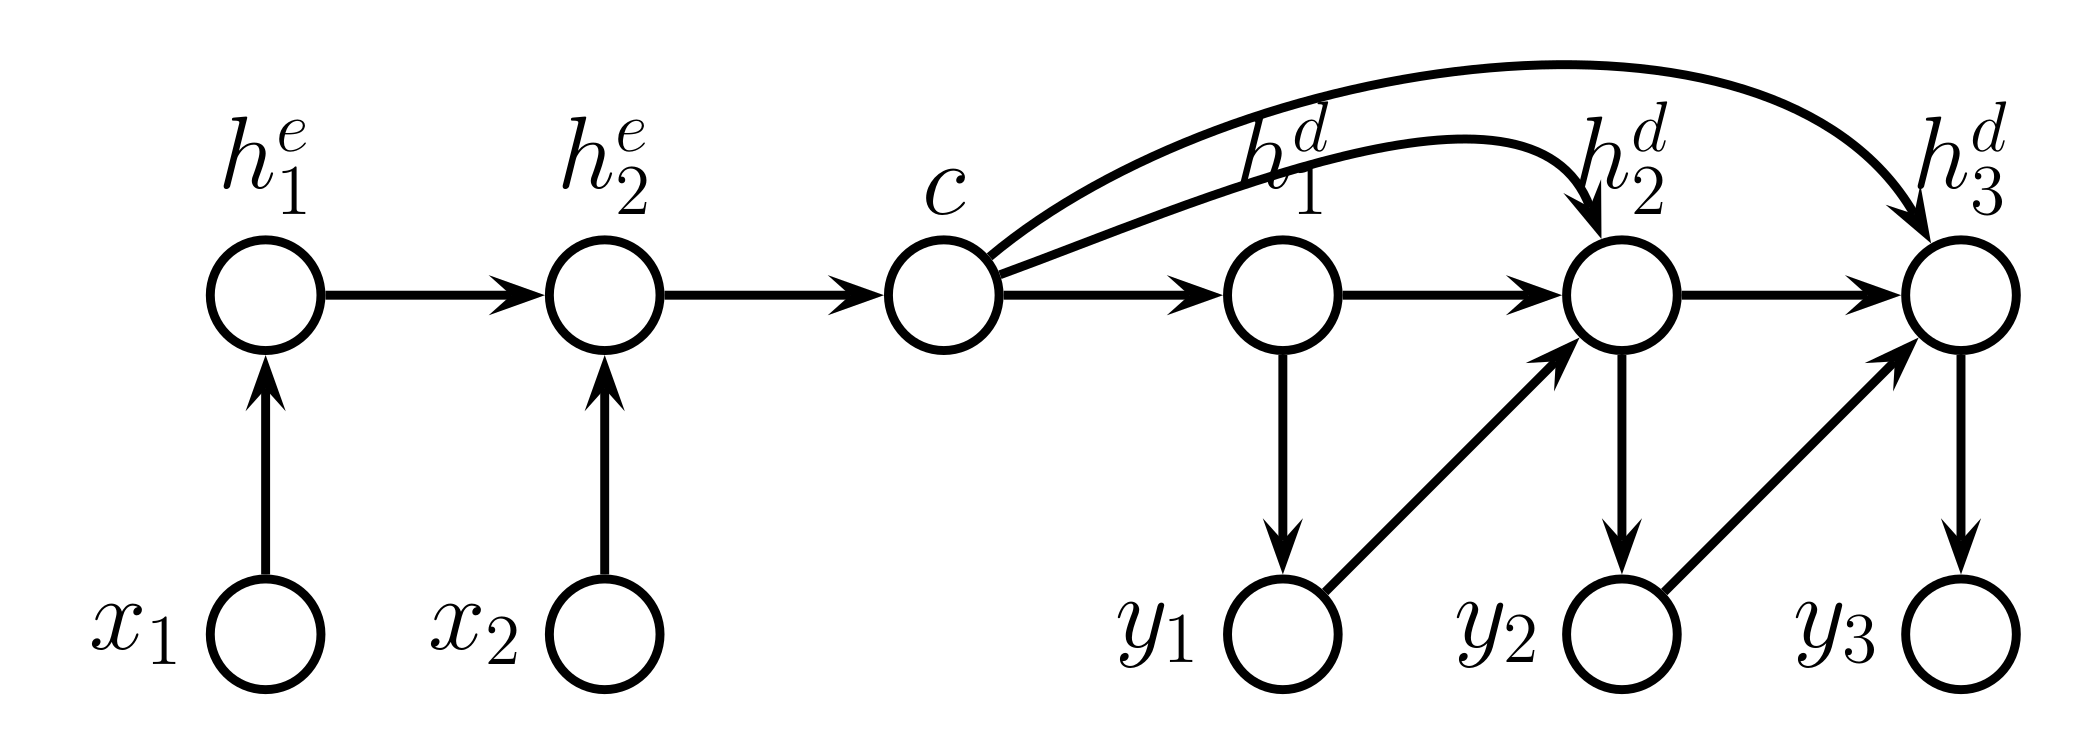
\includegraphics[width=\textwidth]{seq2seq_nonaligned.png} \\

\scriptsize Source: Murphy Fig. 15.7
\end{frame}

\begin{frame}{Recurrent Neural Networks (RNN)}
\begin{itemize}
   \item A neural network block occurs multiple times in sequence
   \item \textbf{Input}: Sequence or single (initial) input
   \item \textbf{Output}: Sequence or single (final) output
   \item \textbf{State}: Hidden, passed from one step to the next
\end{itemize}
\centering
\includegraphics[width=\textwidth]{rnn.png}
\scriptsize \url{https://commons.wikimedia.org/wiki/File:Recurrent_neural_network_unfold.svg}
\end{frame}

\begin{frame}{Backpropagation Through Time}
\begin{align*}
h_t &= \sigma ( W_{x} \cdot x_t + W_{h} \cdot h_{t-1} + B_{h}) \\
o_t &= \sigma (W_{o} \cdot h_t + B_{o} ) 
\end{align*}

\begin{itemize}
   \item Unfolding and truncating to make computationally tractable
   \item Train on short input subsequences
\end{itemize}

\begin{block}{Vanishing Gradient Problem}
\begin{itemize}
   \item Multiplicative updates of state through time
   \item Loss of memory about inputs in distant past
   \item \emph{Solution}: Additive updates of state
\end{itemize}
\end{block}
\end{frame}

\begin{frame}{Long-Short-Term Memory (LSTM) Cells}
\begin{itemize}
   \item ''Input gate'' $I$, ''Forget gate'' $F$, ''Output gate'' $O$, candidate new memory $\tilde{c}_t$
   \item Hidden state $h$, Cell memory $c$
\end{itemize}

\begin{center}
\includegraphics[width=\textwidth]{lstm_wikimedia2.png}
\scriptsize \url{https://en.wikipedia.org/wiki/File:Long_Short-Term_Memory.svg} \normalsize
\end{center}
\end{frame}

\begin{frame}{LSTM Cells}
\begin{align*}
F_t &= \sigma (W_f \cdot [ x_t, h_{t-1}] + b_f) \\
I_t &= \sigma (W_i \cdot [ x_t, h_{t-1}] + b_i) \\
O_t &= \sigma (W_o \cdot [ x_t, h_{t-1}] + b_o) \\[.5\baselineskip]
\tilde{c}_t &= \phi (W_c \cdot [ x_t, h_{t-1}] + b_c) \\[.5\baselineskip]
c_t &= F_t \otimes c_{t-1} + I_t \otimes \tilde{c}_t \\
h_t &= O_t \otimes \phi(c_t) 
\end{align*}

\small
Here $\cdot$ is the dot-product (vector product), $\otimes$ is element-wise multiplication, and $[.]$ denotes vector concatenation. $\sigma$ is the sigmoid/logistic function and $\phi$ is the hyperbolic tangent.
\end{frame}

\begin{frame}{LSTM Cell Parameters}
\small
\begin{itemize}
  \item Let $h_t$ and $c_t$ be vectors of size $n$ and $x_t$ be a vector of size $m$ and 
  \item The input to each gate is of size $n+m$, the output is of size $n$
  \item Then $W_f$, $W_i$, $W_o$ and $W_c$ must be matrices of size $n \times (n+m)$
  \item Then $b_f$, $b_i$, $b_o$ and $b_c$ must be vectors of size $n$. 
  \item Then for each gate there are $n \times (n+m) + n$ parameters
  \item Then for all four gates, there are $4 \times (n \times (n+m) + n)$ parameters
\end{itemize}
\textbf{Important}: Parameters are ''re-used'' for each unrolled step.\\

\textbf{Example}: Let the unit size (state size) be 16 and the input size be 8. Then the total number of parameters for the LSTM cell is $4 \times (16 \times (8+16) + 16) = 1600$
\end{frame}

\begin{frame}{Gated Recurrent Unit (GRU) Cells}
\begin{itemize}
   \item ''Update gate'' $Z$, ''Reset gate gate'' $R$, candidate new memory $\hat{h}_t$
   \item Hidden state $h$
\end{itemize}
\begin{center}
\includegraphics[width=.85\textwidth]{gru_wikimedia.png}
\scriptsize \url{https://en.wikipedia.org/wiki/File:Gated_Recurrent_Unit.svg} \normalsize
\end{center}
\begin{itemize}
   \item Fewer parameters than, and similar performance to LSTM
\end{itemize}
\end{frame}

\begin{frame}{GRU Cells}
\begin{align*}
Z_t &= \sigma (W_z \cdot [x_t, h_{t-1}] + b_z) \\
R_t &= \sigma (W_r \cdot [x_t, h_{t-1}] + b_r) \\[.5\baselineskip]
\hat{h}_t &= \phi (W_h \cdot [x_t, R_t \otimes h_{t-1}] + b_h) \\
h_t &= (1 - Z_t) \otimes h_{t-1} + Z_t \otimes \hat{h}_t
\end{align*}

\small
Here $\cdot$ is the dot-product (vector product), $\otimes$ is element-wise multiplication, and $[.]$ denotes vector concatenation.  $\sigma$ is the sigmoid/logistic function and $\phi$ is the hyperbolic tangent.
\end{frame}

\begin{frame}{GRU Cell Parameters}
\small
\begin{itemize}
  \item Let $h_t$ be a vector of size $n$ and $x_t$ be a vector of size $m$ and 
  \item The input to each gate is of size $n+m$, the output is of size $n$
  \item Then $W_z$, $W_r$, and $W_h$ must be matrices of size $n \times (n+m)$
  \item Then $b_z$, $b_r$, and $b_h$ must be vectors of size $n$. 
  \item Then for each gate there are $n \times (n+m) + n$ parameters
  \item Then for all three gates, there are $3 \times (n \times (n+m) + n)$ parameters
\end{itemize}
\textbf{Important}: Parameters are ''re-used'' for each unrolled step.\\

\textbf{Example}: Let the unit size (state size) be 16 and the input size be 8. Then the total number of parameters for the GRU cell is $3 \times (16 \times (8+16) + 16) = 1200$ \\
{\tiny With Keras GRU layer option \texttt{reset\_after=False}.}
\end{frame}

\begin{frame}{Statefulness of RNN}
\small
\begin{block}{Stateless LSTM/GRU}
\begin{itemize}
   \item Forget internal hidden state and cell memory after each training batch
   \item Allows shuffling of data between epochs
   \item No ''long-term memory'' for the LSTM/GRU
\end{itemize}
\end{block}
\begin{block}{Stateful LSTM/GRU}
\begin{itemize}
   \item Retain internal state and cell memory between training batches
   \item Must not shuffle training data, data must be presented for learning in ''correct'' order
   \item Allows ''long-term memory'' for the LSTM/GRU across multiple batches
\end{itemize}
\end{block}
\end{frame}


\begin{frame}{Hands-On Exercise}

Consider a neural network for regression with the following characteristics:

\begin{itemize}
   \item Layer 1: Embedding
   \begin{itemize}
      \item Embedding matrix: $10000 \times 10$
   \end{itemize}
   \item Layer 2: LSTM (seq2seq)
   \begin{itemize}
      \item Hidden state and cell memory size: 24
      \item Number of unrolled steps: 10
   \end{itemize}
   \item Layer 3: GRU (seq2vec)
   \begin{itemize}
      \item Hidden state size: 16
   \end{itemize}
   \item Layer 4: Dense layer
\end{itemize}

What is the number of trainable parameters for each layer and for the whole network?
\end{frame}


\begin{frame}[fragile]{Stock Market Prediction}
Using historic stock market data, predict future performance.
\begin{itemize}
   \item DJIA performance
   \item ''Seq2Vec'' task: From a sequence of values, predict one following value
   \item Data exported from the R package \texttt{quarks}
   \item 2000 to 2021 (converted to EUR)
   \item Limited to open, low, high, close, and volume data
\end{itemize}
\end{frame}

\begin{frame}[fragile]{Stock Market Prediction \small [cont'd]}
Load packages and read data file:
\begin{pythoncode}
import math
import tensorflow as tf
from tensorflow import keras
from keras import layers
import pandas as pd

tf.random.set_seed(123)
n_steps = 20
n_epochs = 25

data = \
pd.read_csv('https://evermann.ca/busi4720/djia.data.csv')
\end{pythoncode}
\end{frame}

\begin{frame}[fragile]{Stock Market Prediction \small [cont'd]}
Add useful features for timeseries models:
\begin{itemize}
   \item Successive differences
   \item Percentage changes
\end{itemize}
\begin{pythoncode}
data = pd.concat([
    data,
    data.diff().add_suffix('diff'),
    data.pct_change().add_suffix('pct')],
    axis=1).iloc[1:,]
\end{pythoncode}
\end{frame}

\begin{frame}[fragile]{Stock Market Prediction \small [cont'd]}

Split data to train and validation set (no random shuffling for time series):

\begin{pythoncode}
train = data[:math.floor(0.8*data.shape[0])]
valid = data.drop(train.index)
\end{pythoncode}

Normalize data using only info from training set to prevent information 'leakage':

\begin{pythoncode}
train_mean = train.mean()
train_sd = train.std()
train = (train - train_mean)/train_sd
valid = (valid - train_mean)/train_sd
\end{pythoncode}
\end{frame}

\begin{frame}[fragile]{Stock Market Prediction \small [cont'd]}
Create \texttt{tf.Dataset} objects for training and validation:
\begin{pythoncode}
dataset_train = keras.preprocessing \
    .timeseries_dataset_from_array(
        train.drop('price.closediff', axis=1),
        train['price.closediff'],
        sequence_length=n_steps,
        batch_size=32,
        shuffle=True)
\end{pythoncode}

\begin{pythoncode}
dataset_valid = keras.preprocessing \
    .timeseries_dataset_from_array(
        valid.drop('price.closediff', axis=1),
        valid['price.closediff'],
        sequence_length=n_steps,
        batch_size=32,
        shuffle=True)
\end{pythoncode}
\end{frame}

\begin{frame}[fragile]{Interlude -- Dataset Objects}
Dataset objects feed inputs and targets to the \texttt{fit} function. \\

See how this works with simple example data:
\begin{pythoncode}
test = pd.DataFrame([[0, 0], [1, 1], [2, 2,], [3, 3], 
                     [4, 4], [5, 5], [6, 6], [7, 7]]) 
inputs = test.iloc[:-1,0]
targets = test.iloc[2:,1]

pd.DataFrame([inputs, targets])
     0    1    2    3    4    5    6    7
0  0.0  1.0  2.0  3.0  4.0  5.0  6.0  NaN
1  NaN  NaN  2.0  3.0  4.0  5.0  6.0  7.0
\end{pythoncode}
\end{frame}

\begin{frame}[fragile]{Interlude -- Dataset Objects}
Do not shuffle data:
\begin{itemize}
    \item Each batch continues from the previous batch
    \item Suitable for stateful RNN architectures
\end{itemize}

\begin{pythoncode}
ds = keras.preprocessing \
    .timeseries_dataset_from_array(
        inputs, 
        targets,
        batch_size=2, 
        sequence_length=2,
        sequence_stride=1, 
        shuffle=False)
        
for element in ds.as_numpy_iterator():
     print(element)

(array([[0, 1],
       [1, 2]]), array([2, 3]))
(array([[2, 3],
       [3, 4]]), array([4, 5]))
(array([[4, 5],
       [5, 6]]), array([6, 7]))
\end{pythoncode}
\end{frame}

\begin{frame}[fragile]{Interlude -- Dataset Objects}
Shuffle data:
\begin{itemize}
    \item Batches do not continue sequence
    \item Suitable for stateless NN architectures
\end{itemize}

\begin{pythoncode}
ds = keras.preprocessing \
    .timeseries_dataset_from_array(
        inputs, 
        targets,
        batch_size=2, 
        sequence_length=2,
        sequence_stride=1, 
        shuffle=True)
        
for element in ds.as_numpy_iterator():
     print(element)

(array([[4, 5],
       [2, 3]]), array([6, 4]))
(array([[5, 6],
       [0, 1]]), array([7, 2]))
(array([[3, 4],
       [1, 2]]), array([5, 3]))
\end{pythoncode}
\end{frame}

\begin{frame}[fragile]{Interlude -- Dataset Objects}
Sequence stride:

\begin{pythoncode}
ds = keras.preprocessing \
    .timeseries_dataset_from_array(
        inputs, 
        targets,
        batch_size=1, 
        sequence_length=2,
        sequence_stride=2, 
        shuffle=False)
        
for element in ds.as_numpy_iterator():
     print(element)

(array([[0, 1]]), array([2]))
(array([[2, 3]]), array([4]))
(array([[4, 5]]), array([6]))
\end{pythoncode}
\end{frame}

\begin{frame}{Hands-On Exercise -- Dataset Objects}
Using example data as in the previous slides,
\begin{enumerate}
   \item Experiment with different values for \texttt{batch\_size},
   \item Experiment with different values for \texttt{sequence\_length},
   \item Experiment with different values for \texttt{sequence\_stride}.
\end{enumerate}
Do the results match your expectations?
\end{frame}

\begin{frame}[fragile]{Stock Market Prediction \small [cont'd]}
Build a sequential model using an input layer, one LSTM layer and a dense (fully-connected) layer with a single output:
\begin{itemize}
   \item Hidden state and cell memory size: \texttt{units=16}
   \item ''Seq2Vec'' model: \texttt{return\_sequences=False}
   \item Stateless model: \texttt{stateful=False}
\end{itemize}

\begin{pythoncode}
model = keras.Sequential()
model.add(layers.InputLayer(
    input_shape=(n_steps, len(train.columns)-1)))
model.add(layers.LSTM(
    units=16,
    return_sequences=False,
    return_state=False,
    stateful=False))
model.add(layers.Dense(1))
model.summary()
\end{pythoncode}
\end{frame} 

\begin{frame}[fragile]{Stock Market Prediction \small [cont'd]}
Compile the model:
\begin{pythoncode}
model.compile(loss='mean_squared_error', 
              optimizer='Adagrad')
\end{pythoncode}

Fit the model to data:
\begin{pythoncode}
model.fit(dataset_train, epochs=n_epochs, 
          validation_data=dataset_valid)
\end{pythoncode}
\end{frame}

\begin{frame}[fragile]{Stock Market Prediction \small [cont'd]}
Results:
\begin{textcode}
Model: "sequential_4"
_______________________________________________
 Layer (type)       Output Shape     Param #   
===============================================
 lstm_1 (LSTM)      (None, 16)       1984      
 dense_8 (Dense)    (None, 1)        17        
===============================================
Total params: 2001 (7.82 KB)
Trainable params: 2001 (7.82 KB)
Non-trainable params: 0 (0.00 Byte)
_______________________________________________

Epoch 1/25
138/138 [==============================] - 4s 14ms/step 
loss: 1.1351 - val_loss: 7.2034

Epoch 25/25
138/138 [==============================] - 1s 9ms/step
loss: 0.9916 - val_loss: 7.1444
\end{textcode}
\end{frame}


\begin{frame}{Hands-On Exercises}
\small
Download the Python code from \url{https://evermann.ca/busi4720/ts_prediction_s2v_stateless.py}

\begin{enumerate}
   \item Predict the percentage change of the closing value (column \texttt{price.closepct})
   \item Predict the actual closing value (column \texttt{price.close})
   \item Comment on the model performance results. Are these values more or less predictable than the differenced closing values?
\end{enumerate}

Experiment with different model characteristics:
\begin{enumerate}
    \item Vary the size of the LSTM state (\texttt{unit=16}).
    \item Swap the LSTM layer for a GRU layer (\texttt{layers.GRU}). The GRU layer takes the same arguments as the LSTM layer.
    \item Comment on the model performance results.
\end{enumerate}
\end{frame}

\begin{frame}[fragile]{Stock Market Prediction \small [cont'd]}
Can we do better with more layers?
\begin{pythoncode}
model = keras.Sequential()
model.add(layers.InputLayer(
    input_shape=(n_steps, len(train.columns)-1)))
model.add(layers.LSTM(
    units=16,
    return_sequences=True,
    stateful=False))
model.add(layers.Dropout(rate=0.25))
model.add(layers.LSTM(
    units=16,
    return_sequences=False,
    stateful=False))
model.add(layers.Dense(32))
model.add(layers.Dropout(rate=0.25))
model.add(layers.Dense(1))
model.summary()
\end{pythoncode}
The first LSTM returns sequences, the second one does not.
\end{frame}

\begin{frame}[fragile]{Stock Market Prediction \small [cont'd]}
Results of more complex model:
\begin{textcode}
Model: "sequential"
_______________________________________________
 Layer (type)         Output Shape      Param #   
===============================================
 lstm (LSTM)          (None, 20, 16)    2048      
 dropout (Dropout)    (None, 20, 16)    0         
 lstm_1 (LSTM)        (None, 16)        2112      
 dense (Dense)        (None, 32)        544       
 dropout_1 (Dropout)  (None, 32)        0         
 dense_1 (Dense)      (None, 1)         33        
===============================================
Total params: 4737 (18.50 KB)
Trainable params: 4737 (18.50 KB)
Non-trainable params: 0 (0.00 Byte)

Epoch 25/25
138/138 [==============================] - 1s 8ms/step 
- loss: 0.9966 - val_loss: 0.9486
\end{textcode}
\end{frame}

\begin{frame}[fragile]{Stock Market Prediction \small [cont'd]}
Does a stateful LSTM perform better? \\

Set batch size to 1 for a single batch of continuous sequence:
\begin{pythoncode}
dataset_train = keras.preprocessing \
    .timeseries_dataset_from_array(
        train.drop('price.closediff', axis=1),
        train['price.closediff'],
        sequence_length=n_steps,
        sampling_rate=1, batch_size=1, shuffle=False)
\end{pythoncode}

\begin{pythoncode}
dataset_valid = keras.preprocessing \
    .timeseries_dataset_from_array(
        valid.drop('price.closediff', axis=1),
        valid['price.closediff'],
        sequence_length=n_steps,
        sampling_rate=1, batch_size=1, shuffle=False)
\end{pythoncode}
\end{frame}

\begin{frame}[fragile]{Stock Market Prediction \small [cont'd]}
\begin{pythoncode}
model = keras.Sequential()
model.add(layers.InputLayer(
    batch_input_shape=(
        1, None, len(train.columns)-1)))
model.add(layers.LSTM(
    units=16,
    return_sequences=False,
    return_state=False,
    stateful=True))
model.add(layers.Dense(1))
model.summary()
\end{pythoncode}
\end{frame}

\begin{frame}[fragile]{Stock Market Prediction \small [cont'd]}
Results of stateful model:

\begin{textcode}
 Layer (type)    Output Shape    Param #   
=========================================
 lstm (LSTM)     (1, 16)         2048      
 dense (Dense)   (1, 1)          17        
=========================================
Total params: 2065 (8.07 KB)
Trainable params: 2065 (8.07 KB)
Non-trainable params: 0 (0.00 Byte)
_________________________________________
Epoch 1/25
4407/4407 [==============================] 
- 14s 3ms/step - loss: 1.0094 - val_loss: 1.4701

Epoch 25/25
4407/4407 [==============================] 
- 13s 3ms/step - loss: 0.9909 - val_loss: 1.1229
\end{textcode}
\end{frame}

\begin{frame}[fragile]{Hands-On Exercises}
\begin{enumerate}
    \item Download the stateful LSTM from \url{https://evermann.ca/busi4720/ts_prediction_s2v_stateful.py}
    \item Extend the stateful model to a multi-layer network and include dropout layers
    \item How does this change the predictive performance of the model?
\end{enumerate}
\end{frame}

\begin{frame}[fragile]{Stock Market Prediction \small [cont'd]}
How does a ''Vec2Vec'' model perform?

Treat the entire input as one large feature vector, without expressing any time-ordering in the model:
\begin{pythoncode}
model = keras.Sequential()
model.add(layers.InputLayer(
    input_shape=(n_steps, len(train.columns)-1)))
model.add(layers.Flatten())
model.add(layers.Dense(256))
model.add(layers.Dropout(rate=0.25))
model.add(layers.Dense(64))
model.add(layers.Dropout(rate=0.25))
model.add(layers.Dense(1))
model.summary()
\end{pythoncode}
The \texttt{Flatten} layer flattens its input tensor.
\end{frame}

\begin{frame}[fragile]{Stock Market Prediction \small [cont'd]}
Results of ''Vec2Vec'' model. Note the large number of parameters.

\begin{textcode}
 Layer (type)          Output Shape    Param #   
==============================================
 flatten (Flatten)     (None, 300)     0         
 dense (Dense)         (None, 256)     77056     
 dropout (Dropout)     (None, 256)     0         
 dense_1 (Dense)       (None, 64)      16448     
 dropout_1 (Dropout)   (None, 64)      0         
 dense_2 (Dense)       (None, 1)       65        
==============================================
Total params: 93569 (365.50 KB)
Trainable params: 93569 (365.50 KB)
Non-trainable params: 0 (0.00 Byte)

Epoch 1/25  - loss: 3.5692 - val_loss: 2.3847
Epoch 25/25 - loss: 1.5864 - val_loss: 1.0902
\end{textcode}
\end{frame}

\begin{frame}[fragile]{Next Activity Prediction of a Business Process}
\small
Using an event log, train a model to predict the next activity from a prefix sequence of 5 activities that have already occured. \\

Download the complete Python file here: \url{https://evermann.ca/busi4720/process_prediction.py} \\

Download the example event log here: \url{https://evermann.ca/busi4720/BPI_Challenge_2012.xes.gz}

\begin{pythoncode}
import numpy
from tensorflow import keras
from keras import layers
import pandas as pd
import pm4py
# Length of sequences to predict from
prefix_len= 5
# Read the log
log = pm4py.read_xes('BPI_Challenge_2012.xes.gz')
\end{pythoncode}
\end{frame}

\begin{frame}[fragile]{Next Activity Prediction of a Business Process \small [cont'd]}
Fix the data types:
\begin{pythoncode}
log['time:timestamp'] = \
    pd.to_datetime(log['time:timestamp'], utc=True)
log['case:REG_DATE'] = \
    pd.to_datetime(log['case:REG_DATE'], utc=True)
log['case:AMOUNT_REQ'] = \
    pd.to_numeric(log['case:AMOUNT_REQ'])
log['org:resource'] = \
    log['org:resource'].astype(str)
\end{pythoncode}
Filter the log for completion events:
\begin{pythoncode}
# Retain only activity completion events
log = log[log['lifecycle:transition'] == 'COMPLETE']
\end{pythoncode}
\end{frame}

\begin{frame}[fragile]{Next Activity Prediction of a Business Process \small [cont'd]}
Filter and sort the log for sequences of length $k$:
\begin{pythoncode}
# Find the case start time as time of the 
# first event in case
log = log.merge( 
    log.groupby('case:concept:name',as_index=False) \
    ['time:timestamp'].min() \
    .rename(columns={'time:timestamp':'case:start'}), 
    how='left')
# Find the number of events for each case
log = log.merge( 
    log.groupby('case:concept:name', as_index=False) \
    ['time:timestamp'].count(). \
    rename(columns={'time:timestamp':'num_events'}), 
    how='left')
# Filter log for minimum 6 events (5 input, 1 target)
log = log[log['num_events'] > prefix_len]
# Sort log by case start, then by event time
log.sort_values(['case:start', 'time:timestamp'], \
    inplace=True)
\end{pythoncode}
\end{frame}


\begin{frame}[fragile]{Next Activity Prediction of a Business Process \small [cont'd]}
Identify feature to predict from:
\begin{pythoncode}
# This is the feature we predict (from)
f_name = 'concept:name'
# Vocabulary
vocab = list(log[f_name].unique()) + ['EOC']
v_size = len(vocab)
# Dictionaries to convert to/from integers
f2int = dict([(s, vocab.index(s)) for s in vocab])
int2f = dict([(v, k) for (k, v) in f2int.items()])
# Make sequences of feature names for each case
features = log.groupby(['case:concept:name'])[f_name] \
    .apply(list).reset_index(name='features')
\end{pythoncode}
\end{frame}


\begin{frame}[fragile]{Next Activity Prediction of a Business Process \small [cont'd]}
Add end-of-case marker and convert to numeric:
\begin{pythoncode}
sequences=[l+['EOC'] for l in list(features['features'])]
sequences=[[f2int[i] for i in seq] for seq in sequences]
\end{pythoncode}
Split sequences into prefix and target using a sliding window over each sequence:
\begin{pythoncode}
data = pd.DataFrame([(seq[i:i+prefix_len], \
    seq[i+prefix_len]) for seq in sequences \
    for i in range(len(seq)-prefix_len)])
# Split the lists into dataframe columns
data = data.assign(**data[0] \
    .apply(pd.Series).add_prefix('index_'))
\end{pythoncode}
\end{frame}

\begin{frame}[fragile]{Next Activity Prediction of a Business Process \small [cont'd]}
Create training and validation sets:
\begin{pythoncode}
# Divide into train and test set
train = data.sample(frac=0.8)
valid = data.drop(train.index)
# Separate X and Y
train_x = train.iloc[:,2:]
train_y = train.iloc[:,1]
valid_x = valid.iloc[:,2:]
valid_y = valid.iloc[:,1]
\end{pythoncode}
\end{frame}


\begin{frame}[fragile]{Next Activity Prediction of a Business Process \small [cont'd]}
Define the model:
\begin{pythoncode}
model = keras.Sequential()
model.add(layers.InputLayer(input_shape=(5,)))
model.add(layers.Embedding(input_dim=v_size,
                           output_dim=16))
model.add(layers.LSTM(units=32,
                      return_sequences=False,
                      return_state=False,
                      stateful=False))
model.add(layers.Dense(v_size, activation='softmax'))
\end{pythoncode}
Note: \texttt{units} specifies the size of the $h$ and $c$ vectors
\end{frame}

\begin{frame}[fragile]{Next Activity Prediction of a Business Process \small [cont'd]}
Compile and fit the model:
\begin{pythoncode}
# Compile with loss and optimizer
model.compile(loss='sparse_categorical_crossentropy',
              optimizer='Adagrad',
              metrics=['sparse_categorical_accuracy'])
# Train the model and validate on
model.fit(train_x, train_y,
          validation_data=(valid_x, valid_y),
          epochs=25, shuffle=True)
\end{pythoncode}
\end{frame}

\begin{frame}[fragile]{Next Activity Prediction of a Business Process \small [cont'd]}
Results:
\begin{textcode}
 Layer (type)           Output Shape    Param #   
===============================================
 embedding (Embedding)  (None, 5, 16)   384       
 lstm (LSTM)            (None, 32)      6272      
 dense (Dense)          (None, 24)      792                                                                        
===============================================
Total params: 7448 (29.09 KB)
Trainable params: 7448 (29.09 KB)

Epoch 25/25
2875/2875 [==============================] - 6s 2ms/step 
- loss: 1.3819 - sparse_categorical_accuracy: 0.6295 
- val_loss: 1.3825 - val_sparse_categorical_accuracy: 0.6241
\end{textcode}
\end{frame}

\begin{frame}[fragile]{Next Activity Prediction of a Business Process \small [cont'd]}
Predict activities from the model until end-of-case:
\begin{pythoncode}
input = train_x.iloc[2:3,:].copy()
print(input)
probs = model.predict(input)[0]
# pred = probs.argmax()
pred = numpy.random.choice(a=range(v_size), p=probs)
print(int2f[pred])
while int2f[pred] != 'EOC':
    for i in range(4):
        input.iat[0,i] = input.iat[0, i+1]
    input.iat[0,4] = pred
    print(input)
    probs = model.predict(input)[0]
    # pred = probs.argmax()
    pred = numpy.random.choice(a=range(v_size),p=probs)
    print(int2f[pred])
\end{pythoncode}
\end{frame}


\begin{frame}[fragile]{Next Activity Prediction of a Business Process \small [cont'd]}
Results:
\begin{textcode}
       index_0  index_1  index_2  index_3  index_4
109280        6        7        8       10        9
1/1 [==============================] - 0s 197ms/step
W_Nabellen offertes
        index_0  index_1  index_2  index_3  index_4
109280        7        8       10        9        9
1/1 [==============================] - 0s 11ms/step
W_Nabellen offertes
        index_0  index_1  index_2  index_3  index_4
109280        8       10        9        9        9
1/1 [==============================] - 0s 11ms/step
W_Nabellen offertes
        index_0  index_1  index_2  index_3  index_4
109280       10        9        9        9        9
1/1 [==============================] - 0s 11ms/step
EOC
\end{textcode}
\end{frame}


%\begin{frame}[fragile]{Next Activity Prediction of a Business Process \small [cont'd]}
%Alternative model with stacked and bi-directional LSTM:
%\begin{pythoncode}
%model = keras.Sequential()
%model.add(layers.InputLayer(input_shape=(5,)))
%model.add(layers.Embedding(input_dim=v_size,
                           %output_dim=16))
%model.add(
    %layers.Bidirectional(
        %layers.LSTM(units=32,
                    %return_sequences=True,
                    %return_state=False,
                    %stateful=False)))
%model.add(
    %layers.LSTM(units=32,
                %return_sequences=False,
                %return_state=False,
                %stateful=False))
%model.add(layers.Dense(v_size, activation='softmax'))
%\end{pythoncode}
%\end{frame}

\begin{frame}{Hands-On Exercises}
\small
Download the complete Python file here: \url{https://evermann.ca/busi4720/process_prediction.py} \\
Download the example event log here: \url{https://evermann.ca/busi4720/BPI_Challenge_2012.xes.gz} \\

Adapt the network architecture to identify the impact on training and validation performance of the following:
   \begin{enumerate}
      \item Dropouts in the LSTM layer (use the \texttt{dropout=0.x} option when defining the LSTM layer)
      \item GRU instead of LSTM layers (use \texttt{layers.GRU()})
      \item Embedding size (originally 16, note: vocabulary size is 23+1)
      \item Further training epochs (originally 25)
   \end{enumerate}
Comment on your findings and identify the best model. \\
\end{frame}

\end{document}



